
\section{\tikzname{} 互操作}
\label{sec:pgfplots:tikz:interoperability}

\PGFPlots{} 使用 \Tikz{}/\pgfname{} 作为其“后端层”。这意味着它继承了 \Tikz{} 的大多数图形功能，并在其上添加了许多自己的内容。然而，\Tikz{} 和 \PGFPlots{} 的坐标系并不匹配——这是有充分理由的：\PGFPlots{} 操作逻辑（数据）坐标，而 \Tikz{} 操作图像坐标。

偶尔，人们可能希望同步两者以生成图形。在此上下文中，“同步两者”意味着它们真正使用相同的坐标系。这远远超出了“通过 \Tikz{} 注释丰富 \PGFPlots{} 图片”的简单用例，比较 Section~\ref{sec:pgfplots:annotations}。

因此，本节讨论如何将 \Tikz{} 坐标与 \PGFPlots{} 坐标匹配（反之亦然）的问题。它解释如何匹配坐标，并讨论必要的配置。

\PGFPlots{} 中有几个控制坐标映射的键。这些键的目的是实现可视化技术，但它们做的事情与 \Tikz{} 不同（而且应该如此）。要与 \Tikz{} 匹配坐标，需要以下方面：
%
\begin{enumerate}
    \item 限制你的可视化类型：对数坐标轴可能根本不适合 \Tikz{}（更准确地说：它可能适合，但一个 \Tikz{} 单位将对应于 \PGFPlots 中的一个对数单位）。
    \item 通过 |x| 和 |y| 键配置匹配的单位向量。\Tikz{} 的默认配置是使用 |x=1cm,y=1cm,z={(0,0)}|。请注意，这些设置通常被 \PGFPlots{} 覆盖，以遵守 |width| 和 |height|（以及三维坐标轴的 |view|）。
    \item 通过 |disabledatascaling| 禁用数据缩放：\PGFPlots{} 将在内部应用线性坐标变换，以提供浮点运算所需的数据范围（使用近似浮点精度）。禁用数据缩放意味着将自己限制在 \Tikz{} 支持的（小）数据范围内——但在这种情况下，这可能就是你想要的。
    \item 定义 |axis| 的 |anchor| 和位置，可能使用 |anchor=origin,at={(0,0)}|。|at={(0,0)}| 配置 \PGFPlots{} 将坐标轴放置在 \Tikz{} 位置 |(0,0)|，而 |anchor=origin| 意味着 \PGFPlots{} 将其数据原点 $(0,0,0)$ 放置在由 |at| 指定的位置（详情参见 Section~\ref{sec:pgfplots:sec:align}）。
    \item 确保 \PGFPlots{} 坐标轴在显示的数据范围内包含数据原点 $(0,0,0)$（即适当配置 |xmin|、|xmax|、|ymin| 和 |ymax|）。

        没有这一点，上一项所需的 |anchor=origin| 键将被截断为显示范围的下一个坐标。
\end{enumerate}

\noindent 这是一个简单的示例，首先是 \Tikz{}：
%
\begin{codeexample}[]
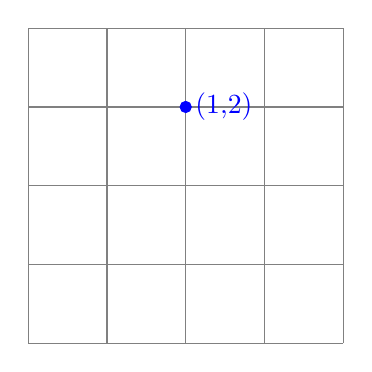
\begin{tikzpicture}
    \coordinate (Point) at (1,2);

    \draw [gray] (-1,-1) grid (3,3);
    \draw [blue,fill] (Point) circle (2pt)
        node [right] {(1,2)}
    ;
\end{tikzpicture}
\end{codeexample}
%
\noindent 它显示一个 $x,y\in[-1,3]$ 的网格，并在其中显示一个节点。
现在，我们应用上面讨论的键来在 \PGFPlots{} 中匹配此设置：
%
\begin{codeexample}[]
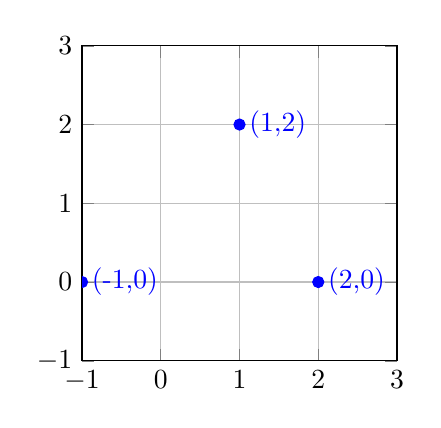
\begin{tikzpicture}
    \coordinate (Point) at (1,2);
\begin{axis}[
    % tell pgfplots to "grab" the axis at its
    % internal (0,0) coord:
    anchor=origin,
    % tell pgfplots to place its anchor at (0,0):
    % (This is actually the default and can
    % be omitted)
    at={(0pt,0pt)},
    % tell pgfplots to use the "natural" dimensions:
    disabledatascaling,
    % tell pgfplots to use the same unit vectors
    % as tikz:
    x=1cm,y=1cm,
    %
    % this is just as usual in pgfplots. I guess
    % it is only useful if (0,0) is part of the
    % range... try it out.
    xmin=-1,xmax=3, ymin=-1,ymax=3,grid=both,
]
    % this uses the point defined OUTSIDE of the axis
    \draw [blue,fill] (Point) circle (2pt)
        node [right] {(1,2)};

    % this uses a TIKZ coordinate (2,0) in the axis:
    \draw [blue,fill] (2,0) circle (2pt)
        node [right] {(2,0)};

    % this here will always work inside of an axis:
    \draw [blue,fill] (-1,0) circle (2pt)
        node [right] {(-1,0)};
\end{axis}
\end{tikzpicture}
\end{codeexample}
%
\noindent 该示例演示了几件事：首先，它在包围的 |tikzpicture| 中定义一个坐标，并在 |axis| 内部使用它（在正确位置）。其次，它在 |axis| 内部使用标准 \Tikz{} 坐标 |(2,0)|，它被放置在预期位置。第三，它使用 \PGFPlots{} 提供的方法，通过使用 |axis cs| 来指定坐标（最后一种方法在没有坐标匹配的情况下也有效）。

这是一个将 \PGFPlots{} 图形正确插入 |tikzpicture| 的示例：
%
% \usepgfplotslibrary{patchplots}
\begin{codeexample}[]
% requires \usepgfplotslibrary{patchplots}
\begin{tikzpicture}
    \begin{axis}[
        % tell pgfplots to "grab" the axis at its internal (0,0) coord:
        anchor=origin,
        % tell pgfplots to place its anchor at (0,0):
        % (This is actually the default and can be omitted)
        at={(0pt,0pt)},
        % tell pgfplots to use the "natural" dimensions:
        disabledatascaling,
        % tell pgfplots to use the same unit vectors as tikz:
        x=1cm,y=1cm,
        %
        hide axis,
    ]
        \addplot [patch,patch type=coons,
            shader=interp,point meta=explicit]
        coordinates {
            (0,0)      [0] % first corner
            (1,-1)     [0] % bezier control point between (0) and (3)
            (4,0.7)    [0] % bezier control point between (0) and (3)
            %
            (3,2)      [1] % second corner
            (4,3.5)    [1] % bezier control point between (3) and (6)
            (7,2)      [1] % bezier control point between (3) and (6)
            %
            (7,1)      [2] % third corner
            (6,0.6)    [2] % bezier control point between (6) and (9)
            (4.5,-0.5) [2] % bezier control point between (6) and (9)
            %
            (5,-2)     [3] % fourth corner
            (4,-2.5)   [3] % bezier control point between (9) and (0)
            (-1,-2)    [3] % bezier control point between (9) and (0)
        };
    \end{axis}

    % this requires pgf 2.10
    \begin{scope}[every node/.style={circle,inner sep=2pt,fill=black}]
        \node [pin=140:first] at (0,0) {};
        \node [pin=second]    at (3,2) {};
        \node [pin=45:third]  at (7,1) {};
        \node [pin=0:fourth]  at (5,-2) {};
    \end{scope}
\end{tikzpicture}
\end{codeexample}
%
\noindent 该示例使用 |patchplots| 库的 |patch| 图之一。由于这些图形元素通常需要深度信息（|z buffer| 缓冲）和颜色数据（|point meta|），它们仅在 \PGFPlots{} 内部可用。然而，上面的配置确保坐标在 \PGFPlots{} 和 \Tikz{} 之间一对一匹配。|hide axis| 标志禁用 \PGFPlots{} 的任何内容，因此只保留可视化的 |patch| 图。\footnote{请注意，\PGFPlots{} 的 $(0,0,0)$ 坐标在此处是数据范围的一部分。}
